% Options for packages loaded elsewhere
\PassOptionsToPackage{unicode}{hyperref}
\PassOptionsToPackage{hyphens}{url}
%
\documentclass[
]{article}
\usepackage{lmodern}
\usepackage{amssymb,amsmath}
\usepackage{ifxetex,ifluatex}
\ifnum 0\ifxetex 1\fi\ifluatex 1\fi=0 % if pdftex
  \usepackage[T1]{fontenc}
  \usepackage[utf8]{inputenc}
  \usepackage{textcomp} % provide euro and other symbols
\else % if luatex or xetex
  \usepackage{unicode-math}
  \defaultfontfeatures{Scale=MatchLowercase}
  \defaultfontfeatures[\rmfamily]{Ligatures=TeX,Scale=1}
\fi
% Use upquote if available, for straight quotes in verbatim environments
\IfFileExists{upquote.sty}{\usepackage{upquote}}{}
\IfFileExists{microtype.sty}{% use microtype if available
  \usepackage[]{microtype}
  \UseMicrotypeSet[protrusion]{basicmath} % disable protrusion for tt fonts
}{}
\usepackage{xcolor}
\IfFileExists{xurl.sty}{\usepackage{xurl}}{} % add URL line breaks if available
\IfFileExists{bookmark.sty}{\usepackage{bookmark}}{\usepackage{hyperref}}
\hypersetup{
  pdftitle={Milestone 8: Replication of `Identifying voter preferences for politicians' personal attributes: a conjoint experiment in Japan'},
  pdfauthor={Evelyn Cai},
  hidelinks,
  pdfcreator={LaTeX via pandoc}}
\urlstyle{same} % disable monospaced font for URLs
\usepackage[margin=1in]{geometry}
\usepackage{longtable,booktabs}
% Correct order of tables after \paragraph or \subparagraph
\usepackage{etoolbox}
\makeatletter
\patchcmd\longtable{\par}{\if@noskipsec\mbox{}\fi\par}{}{}
\makeatother
% Allow footnotes in longtable head/foot
\IfFileExists{footnotehyper.sty}{\usepackage{footnotehyper}}{\usepackage{footnote}}
\makesavenoteenv{longtable}
\usepackage{graphicx,grffile}
\makeatletter
\def\maxwidth{\ifdim\Gin@nat@width>\linewidth\linewidth\else\Gin@nat@width\fi}
\def\maxheight{\ifdim\Gin@nat@height>\textheight\textheight\else\Gin@nat@height\fi}
\makeatother
% Scale images if necessary, so that they will not overflow the page
% margins by default, and it is still possible to overwrite the defaults
% using explicit options in \includegraphics[width, height, ...]{}
\setkeys{Gin}{width=\maxwidth,height=\maxheight,keepaspectratio}
% Set default figure placement to htbp
\makeatletter
\def\fps@figure{htbp}
\makeatother
\setlength{\emergencystretch}{3em} % prevent overfull lines
\providecommand{\tightlist}{%
  \setlength{\itemsep}{0pt}\setlength{\parskip}{0pt}}
\setcounter{secnumdepth}{5}
\usepackage{float}
\let\origfigure\figure
\let\endorigfigure\endfigure
\renewenvironment{figure}[1][2] {
    \expandafter\origfigure\expandafter[H]
} {
    \endorigfigure
}

\title{Milestone 8: Replication of `Identifying voter preferences for politicians' personal attributes: a conjoint experiment in Japan'}
\author{Evelyn Cai}
\date{4/24/2020}

\begin{document}
\maketitle

{
\setcounter{tocdepth}{2}
\tableofcontents
}
~

\hypertarget{abstract}{%
\subsection{Abstract}\label{abstract}}

Horiuchi, Smith, and Yamamoto (2020) found through differences between observational data and their conjoint survey results that Japanese voters' voting preferences are dependent on external factors. The conjoint survey results yielded consistent voter preferences across different levels of knowledge on electoral systems; however, observational data shows that voters' preferences are not consistent in different electoral systems. I was able to successfuly replicate these results and findings. My extension focuses on examining the difference in marginal means instead of the difference of average marginal component effects, which can change the treatment effect estimate.

\pagebreak

\hypertarget{introduction}{%
\subsection{Introduction}\label{introduction}}

~

In Yusaku Horiuchi, Teppei Yamamoto and Daniel Smith's (2020) paper \emph{Identifying voter preferences for politicians' personal attributes: a conjoint experiment in Japan}, they examined observational data from Japanese political candidates and conducted a conjoint survey experiment to determine Japanese voters' attribute preferences and under which circumstances they can be altered. They also explored the effect of a candidate's gender on their electability likelihood and its interaction with other variables, such as awareness of Japan's electoral groups. While it is commonly established that the personal attributes of political candidates do have an impact on voter choice, as they portray in their literature review, they also highlight the fact that certain traits' interaction effects may provide for an explanation for why candidates were chosen (Yusaku Horiuchi (2020)). For example, men were ``awarded'' more for political experience than women, which may explain the severe lack of female representation despite the consistency in gender preferences from the conjoint survey (Yusaku Horiuchi (2020)). They conducted conjoint analyses involving Average Marginal Component Effects (AMCEs) and Average Component Interaction Effects (ACIEs) to determine the effect of different variables on candidate selection likelihood, and whether said variables interacted with each othe in which ways.

~

In replicating their paper and conducting data analysis, I used R, an open source programming language (R Core Team (2019)). All of Horiuchi, Smith, \& Yamamoto's code has been generously made available through the Dataverse.\footnote{Horiuchi, Yusaku; Smith, Daniel M.; Yamamoto, Teppei, 2018, ``Replication Data for: Identifying Voter Preferences for Politicians' Personal Attributes: A Conjoint Experiment in Japan'', \url{https://doi.org/10.7910/DVN/KCIADO}, Harvard Dataverse, V1} All analysis that I have conducted in this exercise can be found at the working Github repository.\footnote{Working repository can be found here: \url{https://github.com/caievelyn/voter_preferences_replication}}

~

With the available code through Dataverse, I was able to replicate the main findings of the paper, which display the AMCEs of different candidate features. The Appendix (see section 0.6) features additional ACIE plots, as well as the mosaic and co-correlation matrices. Charts not include in this replication are additional mosaic plots; the original Appendix had many based off of variables other than age and gender. Similarly, many additional ACIE plots charted the relationship between dynastic politicans and other variables. In the author's original paper and appendix, plots that display analyses using observational data are also present. Diving deeper into the gap between the experimental and observation data, I applied Leeper \emph{et al.}'s (2019) \texttt{cregg} package to the dataset, calculating and displaying the marginal means rather than AMCEs (Thomas J. Leeper (2019)). Marginal means are useful because they avoid setting an arbitrary baseline for comparison, as opposed to AMCEs. This application is significant because the adjusted treatment effect estimates are likely different and could be significantly so.

~

\hypertarget{literature-review}{%
\subsection{Literature Review}\label{literature-review}}

~

Horiuchi, Smith, \& Yamamoto (2020) were also interested in the complexities introduced by the interaction between desired personal attributes and characteristics of election systems. For example, Rule and Zimmerman (1994) found that proportional representation (PR) systems tended to do better in terms of gender parity than first-pass-the-post systems (Wilma Rule (1994)). Additionally, systems that emphasize voting for a candidate as opposed to voting for a party lend more salience to candidates' personal attributes, giving their attributes' desirability (or lack thereof) more weight in the eyes of the voter (JH and DM (2017)). As such, Horiuchi et al.~(2020) wanted to tease out this relationship: Did Japanese voters really prefer male candidates over female candidates at the baseline, or was this preference influenced by characteristics of the system?

~

Japan is a useful case study because of its high ``intra-country variation'' in electoral systems (Wada (2004)). Horiuchi, Smith, \& Yamamoto (2020) tested for whether knowledge of said electoral systems would impact voter preferences using a randomly assigned experiment, and found that there were significant and consistent indications of voter preferences even without priming with knowledge of electoral systems (Yusaku Horiuchi (2020)). They conducted a conjoint survey, in which different candidate attributes were completely randomized and presented for a participant to choose the candidate of their choice. This method of conjoint experiments as applied to political science was popularized by Hainmueller \emph{et al.} (Jens Hainmueller (2014)). Another method employed in the replication paper was compared observational data of actual politicians to the conjoint experiment results. This comparison revealed that the actual representatives in Japan's parliament are very different from the ``ideal'' candidates of the participants, demonstrating that other variables that weren't captured in the conjoint experiment play a large role in elections, such as party candidate recruitment systems (Yusaku Horiuchi (2020)).

~

Horiuchi, Smith, \& Yamamoto (2020) also checked the conjoint data against the actual data of real elected politicians and drew conclusions from the similarities and differences expressed in terms of preferred candidate attributes. Additionally, there were controls for knowledge priming in their conjoint experiment. A control group had no sort of priming about Japan's electoral systems, whereas a treatment group was primed with knowledge about Japan's electoral systems (such as the relationship between voting for a party and proportional representation). They found that there was only one of 56 statistically significant differences in attribute preferences. However, interestingly enough, the actual observations of elected candidates do reveal that there is a discrepancy in the type of candidate elected when constituents are aware of how electoral systems function versus when they are unaware. To parse out the interaction effects of features such as experience and age with the gender variable, the authors calculated ACIEs for the gender variable. The results are displayed below, and reveal that male and female candidates are in fact rewarded/ punished differently based on gender. This finding facilitated the authors' conclusion that external factors, such as party recruitment tactics, are key in influencing voter preferences, rather than electoral systems directly influencing voter preferences as a nature of their configurations.

\begin{figure}
\centering
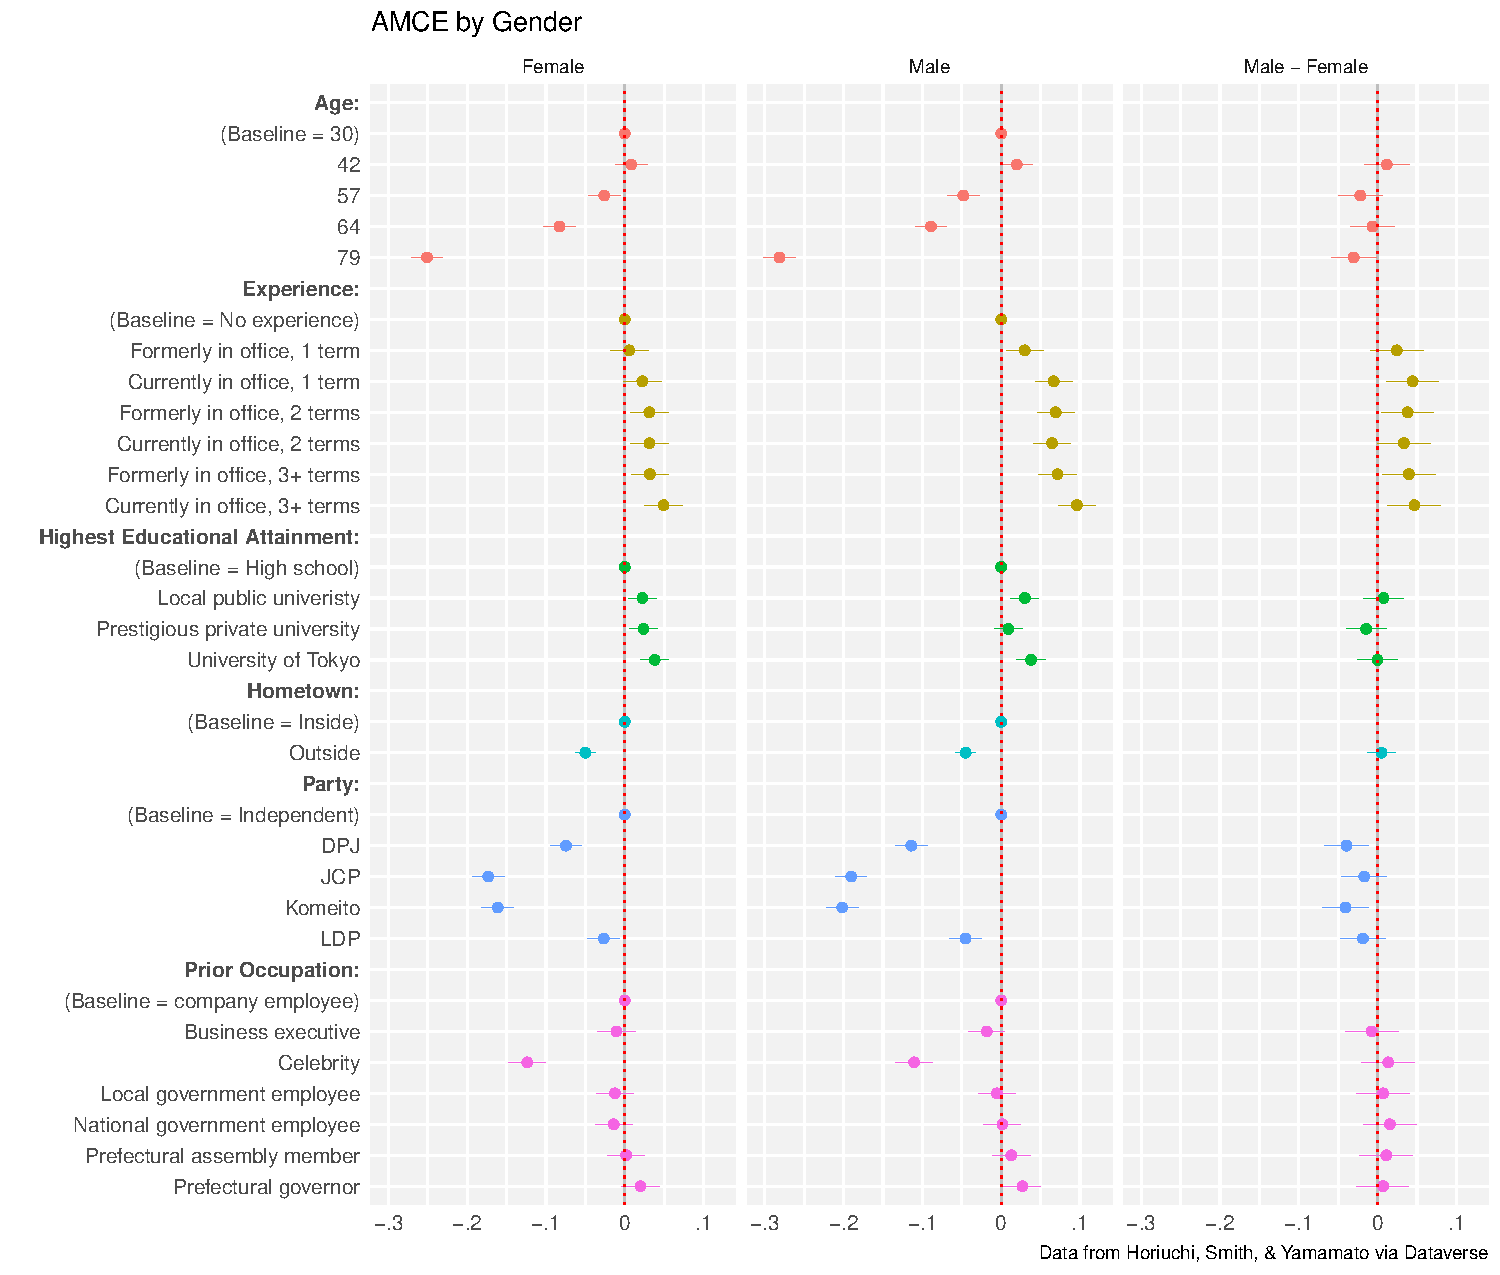
\includegraphics{milestone_8_files/figure-latex/display-1.pdf}
\caption{\label{fig:display}The first two columns on the left display the average treatment effects for different variables, keeping the gender of the candidate constant. The third column displays the difference in average treatment effect, subtracting that of males to that of females. As you can see, party and age have large effects on candidate selection. However, when taking the different in AMCEs, there is no substantial difference between traits that are desired in male and female candidates. The average treatment effect can be interpreted as the `boost' a certain characteristic gives a candidate; negative values indicate hurting the candidate's chances of being chosen, while positive values reflect desirable traits.}
\end{figure}

\hypertarget{replication}{%
\subsection{Replication}\label{replication}}

Thanks to the available data and code, written primarily in base R, I was able to replicate the main findings. The key differences in the provided data and my processing code is the use of \texttt{tidyverse} packages. Tidyverse is a library that collects various open-source packages, which make data cleaning, analysis, and visualization much easier (Wickham et al. (2019)). For example, in constructing the conjoint analyses plots, I utilized the \texttt{cregg} package developed by Thomas Leeper, which automatically combines the calculation of AMCEs, MMs, and more, and \texttt{ggplot2} plotting functionalities. Thank you to the authors for their clean, easily replicable code!

\hypertarget{extension}{%
\subsection{Extension}\label{extension}}

~

According to Leeper \emph{et al.} (2019), a flaw with interpreting ``differences in conditional AMCEs as differences in underlying preferences'' exists because of how the subgroups that are being compared are chosen, and whether there are any meaningful \emph{absolute} differences (Thomas J. Leeper (2019)). Finding the marginal means, then, are useful because there are no baseline values for comparison, but rather allows all variable levels to be compared in a relative sense.

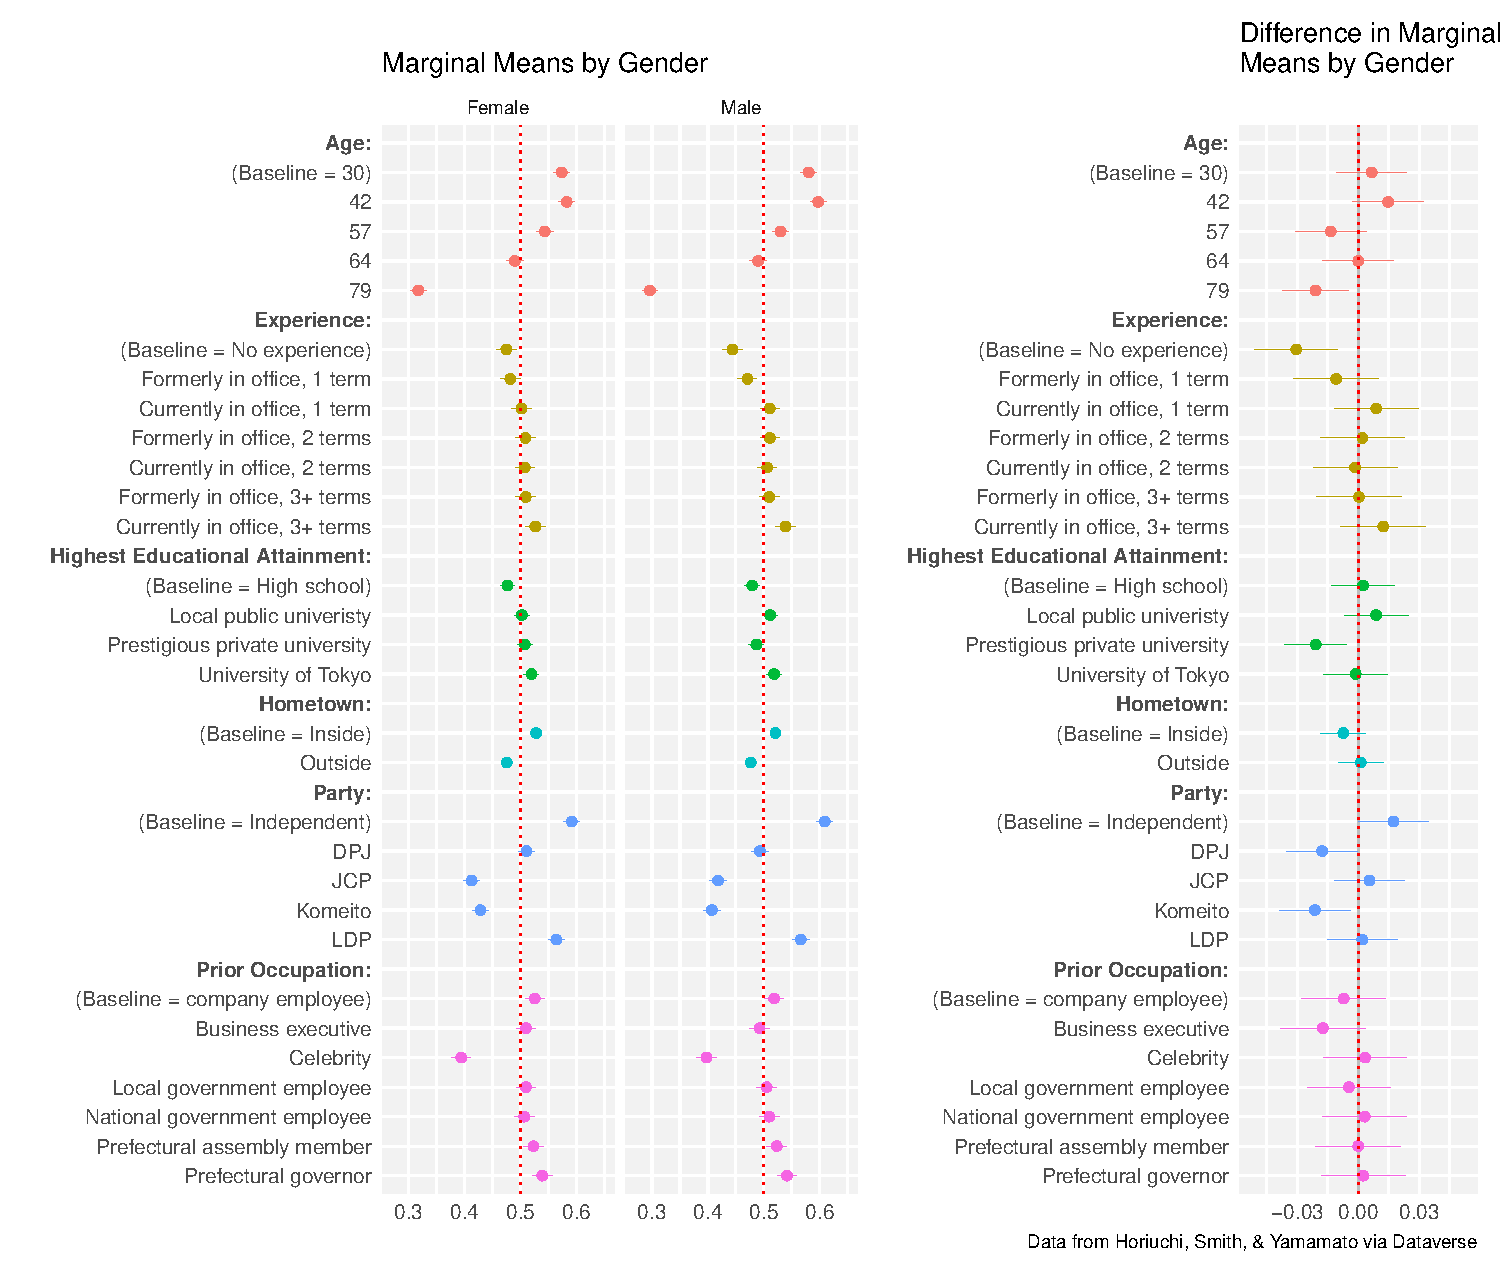
\includegraphics{milestone_8_files/figure-latex/display_2-1.pdf}

\emph{Figure 2}: The top graphic displays the marginal means graph. As you can see, notable differences between the genders include the effect of political experience. Interestingly, in the marginal means graph (we shall denote them as MM graphs), the baseline of ``No experience'' seems to punish men more so than women. This is interesting because women are more likely than men to be part of dynastic political families, and supports the notion that young first-timer female candidates hit a so-called ``bamboo ceiling'' as their political careers lengthen, according to Horiuchi \emph{et al.} (Yusaku Horiuchi (2020)).

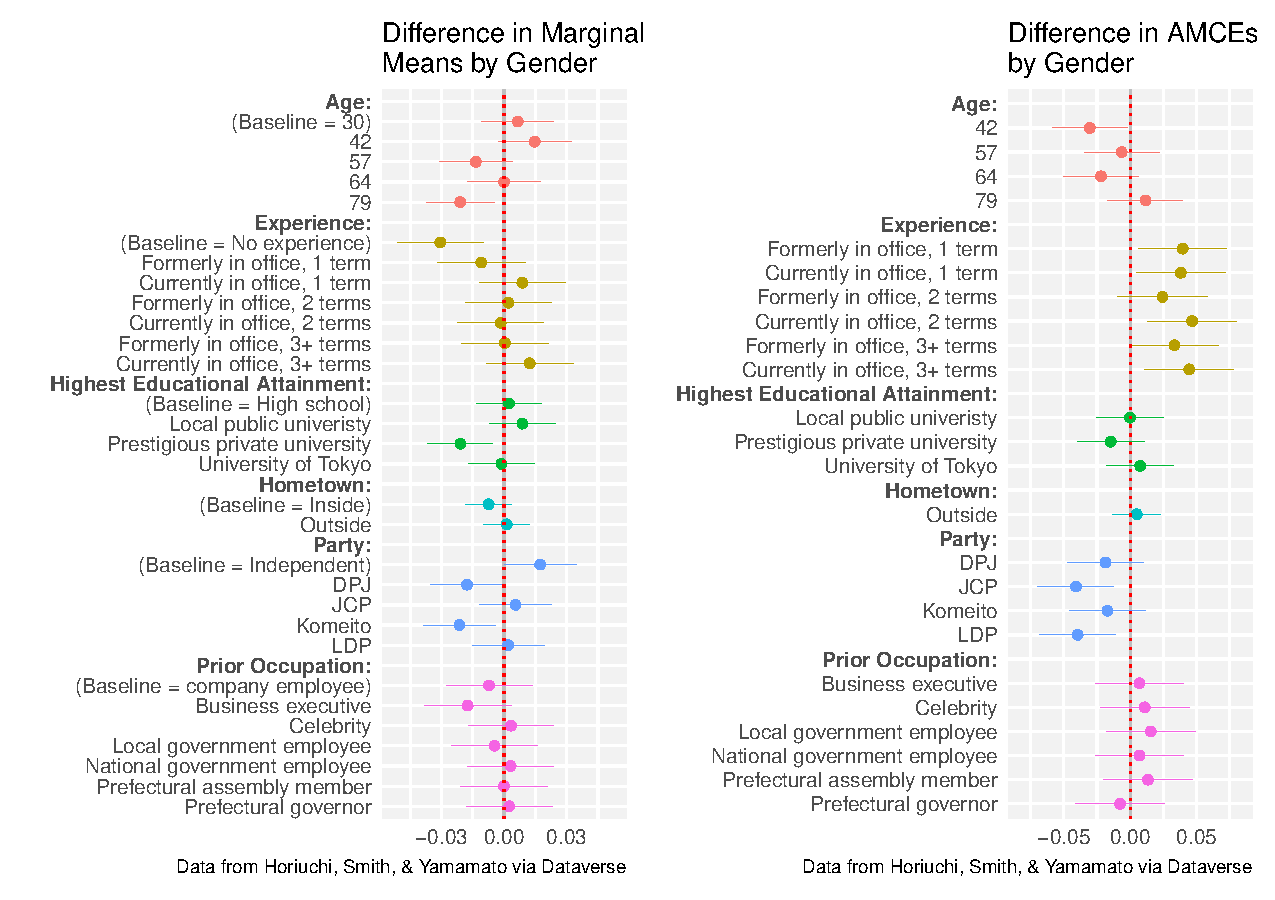
\includegraphics{milestone_8_files/figure-latex/display_3-1.pdf}

\emph{Figure 3}: Side-by-side comparison of the marginal means differences graph and the difference in AMCE graph.

\hypertarget{conclusion}{%
\subsection{Conclusion}\label{conclusion}}

~

Through this replication of Horiuchi, Smith, \& Yamamoto's (2020) paper, I was able to replicate their main findings. There were significant voter preferences consistent even across the treatment and control groups, which received information regarding different electoral systems. Some of these observations include a preference for non-celebrity candidates, candidates from within the prefecture, and younger political candidates. There was no gender preference, all other attributes held equal.

~

However, observational data contradicts these consistent preferences found in conjoint analyses; Japan has a persistently unequal parliamentary body. To make sense of this gap, the authors investigated the ACIE of specific variables, namely the gender variable. Importantly, they found that women received less of a reward in voters' eyes for having more experience, relative to their male counterparts. As such, Horiuchi, Smith, \& Yamamoto (2020) looked at external explanations, such as party recruitment tactics, to account for the legislative gender inequality and gap between experimental and observational data.

~

My extension of the paper looked at marginal means instead of AMCEs. I was most interested in comparing the difference in marginal means for female and male candidates against the difference in AMCEs for female and male candidates.

\hypertarget{appendix}{%
\subsection{Appendix}\label{appendix}}

~

Results from Horiuchi, Smith, \& Yamamoto (2020) were successfully replicated. As an example, here is Figure A.1 from page 2 of the online Appendix. Below it is the co-correlation matrix as displayed on Page 7 of the online Appendix.

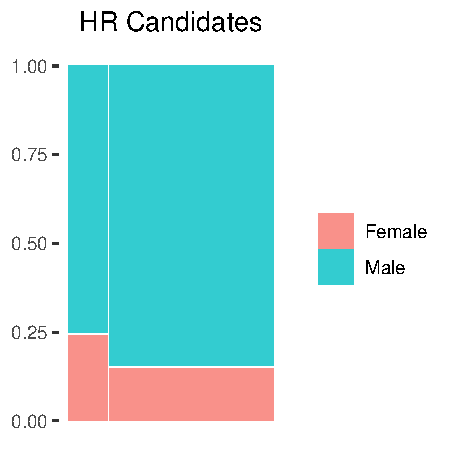
\includegraphics{milestone_8_files/figure-latex/mosaic-1.pdf} 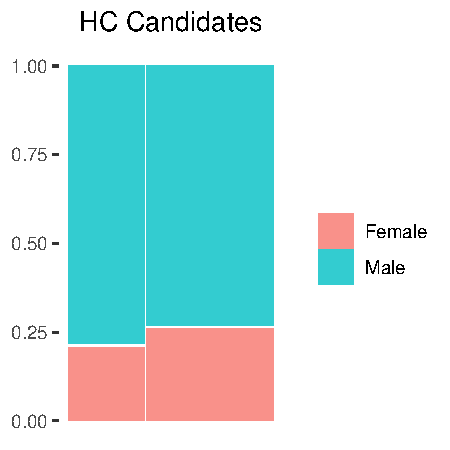
\includegraphics{milestone_8_files/figure-latex/mosaic-2.pdf} 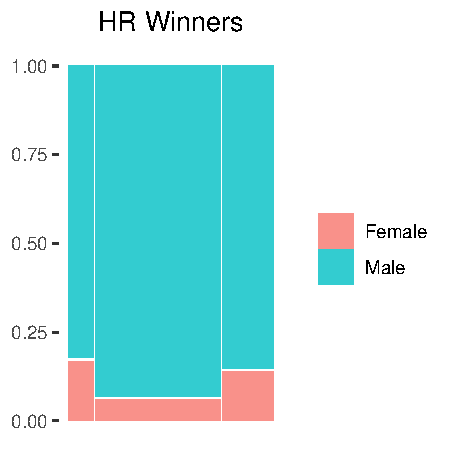
\includegraphics{milestone_8_files/figure-latex/mosaic-3.pdf} 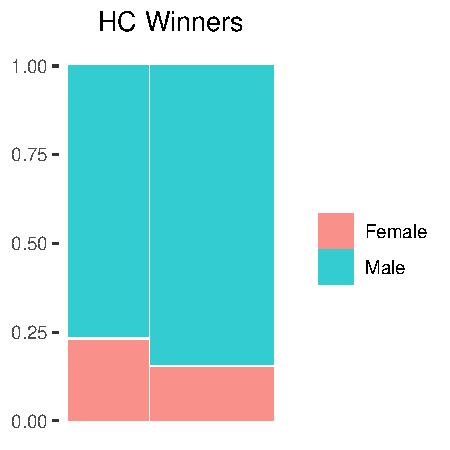
\includegraphics{milestone_8_files/figure-latex/mosaic-4.pdf} 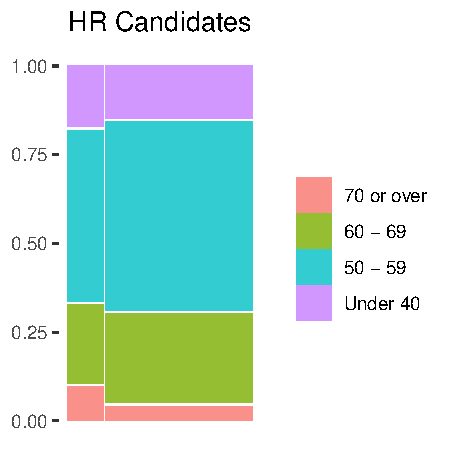
\includegraphics{milestone_8_files/figure-latex/mosaic-5.pdf} 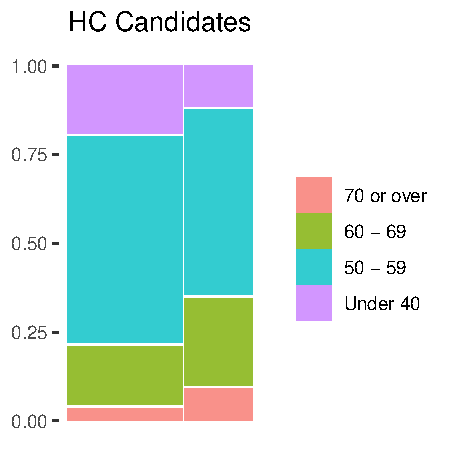
\includegraphics{milestone_8_files/figure-latex/mosaic-6.pdf} 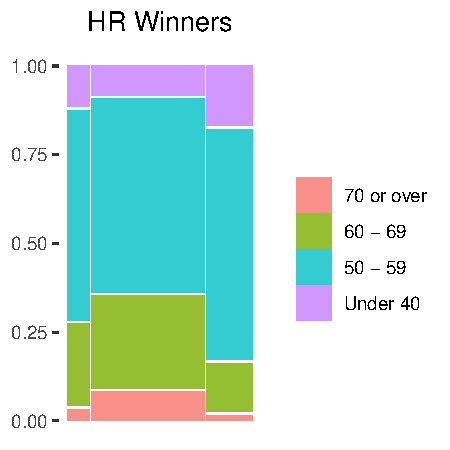
\includegraphics{milestone_8_files/figure-latex/mosaic-7.pdf} 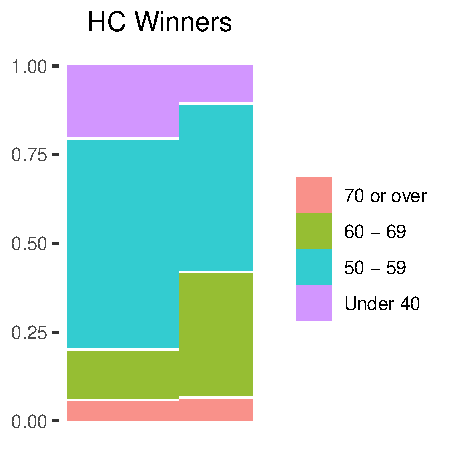
\includegraphics{milestone_8_files/figure-latex/mosaic-8.pdf}

\emph{Figure 4}: The above eight mosaic plots subset by gender and age. HR represents House of Representatives, the lower chamber of Japanese parliament, whereas HC represents the House of Councillors, the upper chamber of Japanese parliament. The figures also compare the share of candidates that ran in SNTV (multi-member)/PR districts versus the proportion of winners from either district.

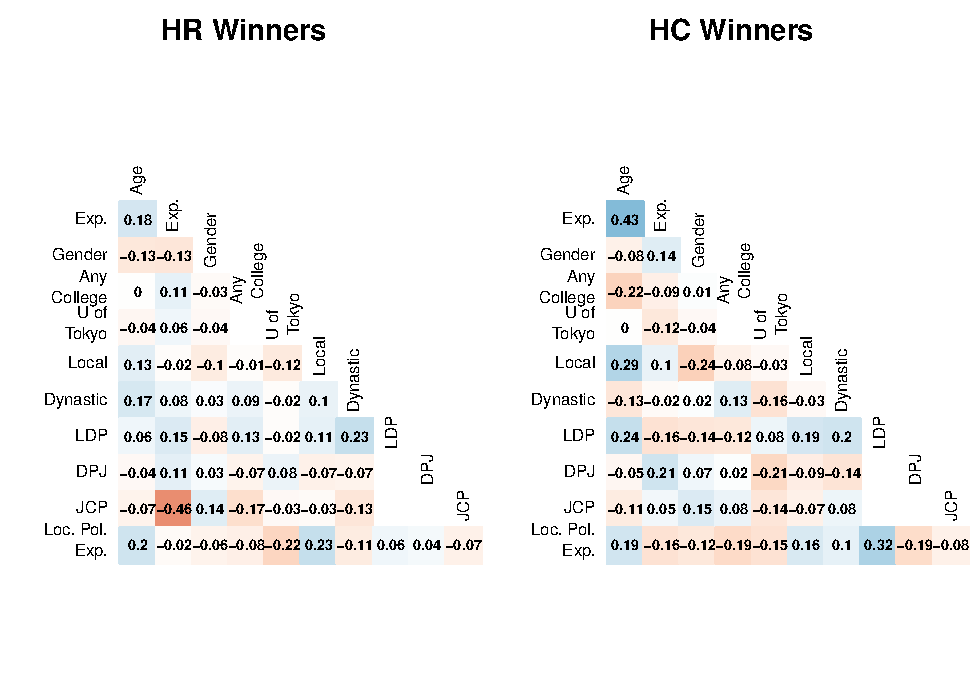
\includegraphics{milestone_8_files/figure-latex/correlation_matrix-1.pdf}

\emph{Figure 5}: Co-correlation matrix providing the correlation coefficients between two variables. Negative values are shaded in red and positive values are shaded in blue. The intensity of the color corresponds to the magnitude of the correation coefficient.

\hypertarget{bibliography}{%
\subsection*{Bibliography}\label{bibliography}}
\addcontentsline{toc}{subsection}{Bibliography}

\hypertarget{refs}{}
\leavevmode\hypertarget{ref-R-conjointmethod}{}%
Jens Hainmueller, Teppei Yamamoto, Daniel J. Hopkins. 2014. ``Causal Inference in Conjoint Analysis: Understanding Multidimensional Choices via Stated Preference Experiments.'' \emph{Political Analysis} 22 (January): 1--30. \url{https://www.cambridge.org/core/journals/political-analysis/article/causal-inference-in-conjoint-analysis-understanding-multidimensional-choices-via-stated-preference-experiments/414DA03BAA2ACE060FFE005F53EFF8C8}.

\leavevmode\hypertarget{ref-R-salience}{}%
JH, Fiva, and Smith DM. 2017. ``Local Candidates and Voter Mobilization: Evidence from Historical Two-Round Elections in Norway.'' \emph{Electoral Studies} 45 (February): 130--40. \url{https://biopen.bi.no/bi-xmlui/handle/11250/2437708}.

\leavevmode\hypertarget{ref-R}{}%
R Core Team. 2019. \emph{R: A Language and Environment for Statistical Computing}. Vienna, Austria: R Foundation for Statistical Computing. \url{https://www.R-project.org/}.

\leavevmode\hypertarget{ref-leeper}{}%
Thomas J. Leeper, James Tilley, Sara B. Hobolt. 2019. ``Measuring Subgroup Preferences in Conjoint Experiments.'' \emph{Political Analysis} 28 (April): 207--21. \url{https://www-cambridge-org.ezp-prod1.hul.harvard.edu/core/journals/political-analysis/article/measuring-subgroup-preferences-in-conjoint-experiments/4F2C21AC02753F1FFF2F5EA0F943C1B2}.

\leavevmode\hypertarget{ref-electoral}{}%
Wada, Junichiro. 2004. ``Japan: Manipulating Multi-Member Districts - from Sntv to a Mixed System.'' In \emph{The Handbook of Electoral System Choice}, edited by Josep M. Colomer, 512--29. London: Palgrave Macmillan UK. \url{https://doi.org/10.1057/9780230522749_30}.

\leavevmode\hypertarget{ref-tidyverse}{}%
Wickham, Hadley, Mara Averick, Jennifer Bryan, Winston Chang, Lucy D'Agostino McGowan, Romain François, Garrett Grolemund, et al. 2019. ``Welcome to the tidyverse.'' \emph{Journal of Open Source Software} 4 (43): 1686. \url{https://doi.org/10.21105/joss.01686}.

\leavevmode\hypertarget{ref-gender}{}%
Wilma Rule, Joseph Francis Zimmerman. 1994. \emph{Electoral Systems in Comparative Perspective: Their Impact on Women and Minorities}. Greenwood Publishing Group.

\leavevmode\hypertarget{ref-R-yamamoto}{}%
Yusaku Horiuchi, Teppei Yamamoto, Daniel M. Smith. 2020. ``Identifying Voter Preferences for Politicians' Personal Attributes: A Conjoint Experiment in Japan.'' \emph{Political Science Research and Methods} 8 (January): 75--91. \url{https://www-cambridge-org.ezp-prod1.hul.harvard.edu/core/journals/political-science-research-and-methods/article/identifying-voter-preferences-for-politicians-personal-attributes-a-conjoint-experiment-in-japan/95ADB2B43C5289ECFE6898B7FE776CFE}.

\end{document}
